%!TEX root = ../dissertation.tex

\chapter{State of the art}
\label{chapter:stateoftheart}

The objective of the present work is to assess the performances of a system that provides situational awareness to rescuers during a wildfire. The main evaluation tool is a simulation. The envisioned system is based on two main ideas: the deployment of \glspl{UAV} to dynamically provide network coverage to ground nodes and the usage of the LoRa technology as \gls{AtG} communication protocol. In order to establish a background of notions that can support and contextualize the contributions given in the present work, the state of the art is presented in this chapter. The main studies and results regarding LoRa and its performance are first described. The main network simulators and the available LoRaWAN simulation modules, with their characteristics, advantages and drawbacks are discussed next. Finally, the most relevant centralized and distributed \gls{UAV} swarm mobility models are presented.


\section{Performance Assessments of LoRa and LoRaWAN}

LoRa is a relatively recent technology. The first patent for the LoRa modulation was issued in 2008, while the first version of the LoRaWAN standard was released only in June 2015. Even if it is a young technology, LoRa got the attention of both the academy and the general public, especially thanks to the availability in the market of cheap LoRa \glspl{ED} and \glspl{GW}. \gls{TTN} is a notable example of a global LoRaWAN network that is continuously expanded and supported by the members of the community. As of today, \gls{TTN} consists of more than 3500 active gateways deployed all around the world and gives the opportunity to the users to deploy their devices and build their applications. LoRa also got the attention of many researchers. As a result, a vast literature focusing on various aspects of the technology has been produced in the last couple of years. \\ \\
Petajajarvi et al. \cite{ref:soa-lora-range1} have conducted empirical measures to determine the maximum range of LoRa in a small rural city in Finland. The results show that, by using the maximum \gls{SF} and a bandwidth of 125 kHz in the 868 MHz band, the signal can reach the \gls{GW} from 15 Km of distance on ground and 30 Km on water, with increments in the \gls{PDR} proportional to the distance. Jörke et al. \cite{ref:soa-lora-range2} have performed a similar analysis in a medium density urban area, noting in this case, that the maximum range under the same conditions described in \cite{ref:soa-lora-range1} is only 5.8 Km, mainly due to the presence of obstacles in the \gls{LOS}. In \cite{ref:soa-lora-range3}, the reception in presence of indoor \glspl{ED} is also evaluated: the authors report that at a distance of 1.2 Km from the gateway, the \gls{PDR} is already between 60\% and 90\%. The conclusion of the authors is that the presence of \gls{LOS} is particularly important. The conclusion is that LoRa is not suited for indoor environments if long range and low \gls{PDR} are required. The importance of \gls{LOS} is also outlined by Iova et al. \cite{ref:soa-lora-mountains}. In this case the experiments were conducted in a forest in presence of numerous trees between the transmitter and the receiver. In the experiment, the transmitter was moved further and further away from the receiver and at around 90-100 m the signal was completely lost. The authors conclude that vegetation has a huge impact on LoRa signal propagation by dropping the range of an order of magnitude. \\ \\
The use of \gls{CSS}, a variation of \gls{DSSS}, makes the LoRa modulation very resilient to noise. This assumption is verified by Angrisani et al. \cite{ref:soa-lora-noise}. In the experiment, different levels of white Gaussian noise were applied to the signal starting with a minimum SNR of -10 dBm. As expected, the use of a smaller bandwidth and, more significantly, the use of a higher \gls{SF} improves the performance of the modulation. The coding rate, on the other hand, has a less significant impact on the performance in noisy environments. \\ \\
One of the main requirements of an \gls{LPWAN} is its ability to scale to hundreds or even thousands of devices. Early attempts of assessing the scalability of LoRa were performed by resorting to mathematical models. Mikhaylov et al. \cite{ref:soa-lora-scal1} assessed the scalability of a LoRa network in presence of a single \gls{GW}. The authors modelled the LoRaWAN MAC as pure ALOHA and reached the conclusion that LoRa can potentially scale to millions of devices in case of \glspl{ED} generating only intermittent uplink traffic, but most of the devices need to be positioned very close to the \gls{GW}. This means that only a limited set of \glspl{ED} can take advantage of the range boost given by higher \glspl{SF}. The authors also point out that huge scalability issues are present in downlink, since \glspl{GW} are still subject to duty cycle limitations and acknowledging every uplink packet of a large network is 	impossible. Augustin et al. \cite{ref:soa-lora-scal2} considered a single LoRaWAN logical channel, characterized by the couple $<frequency,\ SF>$, and performed some simulations assuming Poisson packet arrivals, packet payloads uniformly distributed between 1 and 51 bytes and a 1\% duty cycle. The authors conclude that LoRaWAN behaves almost exactly like ALOHA, in fact the maximum capacity usage is 18\% with a load factor of 0.48.
Bor et al. \cite{ref:soa-lora-scal3} developed LoRaSim, a collision simulator that supports multiple \glspl{GW} and models the capture effect, i.e. the effect that cause a signal that is received with more power to be correctly decoded even if overlapping with other interfering signals. A more detailed description of the simulator features is given is Section \ref{sec:lora-sim}. The authors used LoRaSim to conduct a series of experiments consisting in measuring the Data Extraction Rate (DER), defined as the ratio between the received packets and the transmitted packets, as a function of the number of deployed \glspl{ED}. In the first experiment the DER is measured for the three different transmitter configurations shown in Table \ref{tab:lorasim1}.


\begin{table}[tph]
\centering
\begin{tabular}{|c|c|c|c|}
\hline
Parameter &  $SN^1$ & $SN^2$ & $SN^3$\\ \hline
 Tx Power (dBm) & 14 & 14 & 14  \\ \hline
 Center frequency (MHz) & 868 & 868 & 868 \\ \hline
 \gls{SF} & 12 & 6 & 12  \\ \hline
 Bandwidth (kHz) & 125 & 500 & 125  \\ \hline
 Coding Rate & 4/8 & 4/5 & 4/5 \\ \hline 
 Packet arrival rate & $1 \times 10^{-6}$ & $1 \times 10^{-6}$ & $1 \times 10^{-6}$  \\ \hline
\end{tabular}
\caption{\glspl{ED} PHY configurations used in the experiments performed in \cite{ref:soa-lora-scal3}}
\label{tab:lorasim1}

\end{table}

\begin{figure}[tph]
    \centering
    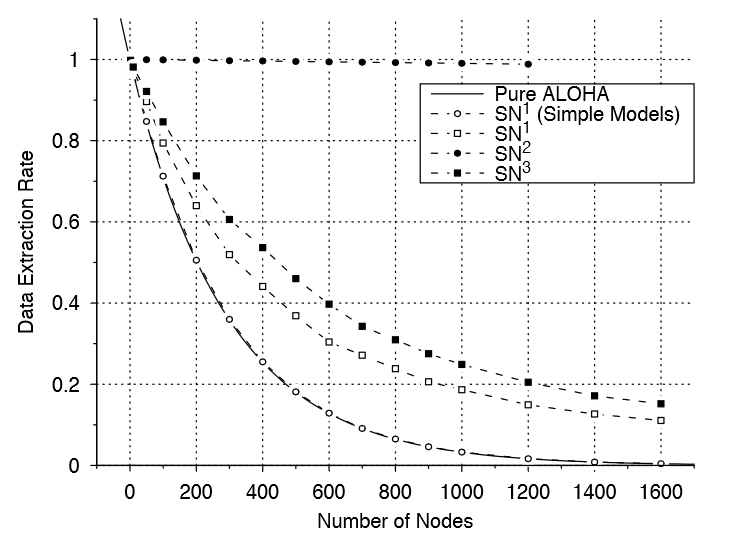
\includegraphics[width=0.8\textwidth]{images/lorasim1.png}
    \caption{Fraction of correctly received packets with one \gls{GW} and a varying number of \glspl{ED} having different PHY configurations \cite{ref:soa-lora-scal3}}
    \label{fig:lorasim1}
\end{figure}

\begin{figure}[tph]
    \centering
    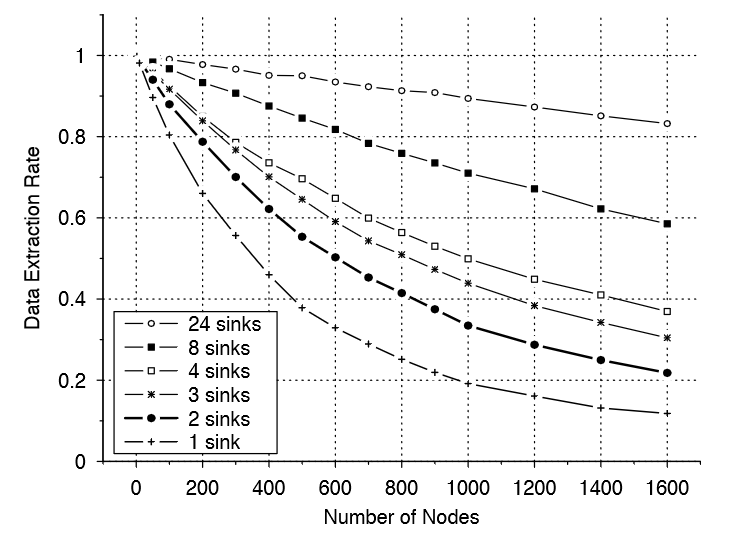
\includegraphics[width=0.8\textwidth]{images/lorasim2.png}
    \caption{Fraction of correctly received packets with multiple \glspl{GW} and a varying number of \glspl{ED} \cite{ref:soa-lora-scal3}}
    \label{fig:lorasim2}
\end{figure}

As shown in Figure \ref{fig:lorasim1}, the results confirm that LoRaWAN behaves exactly like ALOHA with the simple collision assumption of \cite{ref:soa-lora-scal2}. However, with the more realistic collision model of LoRaSim, LoRaWAN performs better than ALOHA in typical \gls{SF} 12 configurations. The authors suggest that ALOHA can be used as a good lower bound estimation of the LoRaWAN behaviour. A second experiment, using $SN^1$ and a varying number of \glspl{GW} produced the results depicted in Figure \ref{fig:lorasim2}. As it is noticeable, the presence of multiple \glspl{GW} can significantly increase the number of supported \glspl{ED} having $DER \geq 0.9 $.

%An effective solution to dynamically adapt the parameters of \glspl{ED} in order to increase the network capacity is presented by Cuomo et al. \cite{ref:soa-lora-scal6}. Two algorithms of increasing complexity, EXPLoRa-SF and EXPLoRa-AT, have been developed to dynamically assign the \gls{SF} to \glspl{ED} based on distance from the \gls{GW}, RSSI and number of connected devices. The results of the simulations conclude that these approaches significantly outperform the basic \gls{ADR} algorithm.
%http://flora.aalto.fi/download/slabicki2018adaptive.pdf  Cite also this maybe 

\section{Network Simulators and LoRaWAN Implementations}
\label{sec:lora-sim}
In order to study different aspects of a complex network or system, researchers have always resorted to one of three methods: theoretical analysis, simulations or experiments using prototypes. Simulations are on the middle ground with respect to the other methods, since they offer a theoretically accurate and cost-effective environment to test how complex systems behave and interacts with one another. One of the most well known open source general purpose network simulators is ns-3. \\\\
ns-3, acronym that stands for network simulator 3, is a discrete event simulator built in C++. Its principal purpose is the simulation of networks based on the IP protocol, even if multiple modules are available to simulate also non-IP networks. ns3 is highly modular and allows for an easy integration of different network models that can be linked together in a very easy and flexible way. This modularity allows the usage of already existing well tested and well document models to build new functionalities or simulation scripts. In terms of performance, as it is pointed out by Weingartner et al. \cite{ref:soa-ns-comp}, ns-3 is one of the best simulators in terms of speed and memory usage.
ns-3 is a discrete event simulator. As such, all the events that may arise in the network (e.g. sending/reception of a packet) are previously determined and scheduled for execution at a specific time. When the simulation start, the scheduled events start being executed in order until the last event is completed. During the simulation, new events can be dynamically added to the scheduler. In ns-3 it's possible to distinguish the following basic components:

\begin{itemize}
	\item \textit{Nodes:} they are abstractions of the physical devices that form the network (e.g. mobile phones, PCs, sensors) and they are instances of the \textit{Node} class. When they are instantiated, they are just empty containers in which it's possible to install applications, net devices, protocols, etc.
	
	\item \textit{Application:} abstractions of the applications running on the network devices. They give the ability to the devices to perform particular tasks, for example sending or receiving UDP packets. Every application is an instance of the \textit{Application} class that has been specialized by the author of the application in order to perform a certain function;
	
	\item \textit{Channels:} a network needs some sort of connection among the devices. The connection can be physical (e.g. an Ethernet cable) or wireless. In ns-3 all these connections are modelled with a specialization of the \textit{Channel} class;
	
	\item \textit{Net Devices:} in the simulator logic, they substitute Network Interface Cards (NIC) and the drivers necessary to operate the network. They allow a node to communicate to another node through a channel. Every net device is a specialization of the \textit{NetDevice} class;
	
	\item \textit{Helpers:} tools that simplify the process of creating a network by providing specific methods to create set of nodes, install net devices and channels and configure the protocol stack.
	
\end{itemize}

ns-3 implements also some systems to collect and analyse the data generated by the simulation:

\begin{itemize}
 \item \textit{Logging module:} this module allows to display messages in the terminal during the execution of the simulation. The logging module is organized in levels, ordered based on an increasing level of verbosity. The logging module can be enabled for all the components of the simulation or only for some modules;
 \item \textit{Tracing System:} the logging module is useful during the debugging phase, but it's inefficient when the real simulation is executing. For this reason, ns-3 implements a tracing system based on the concepts of tracing source and tracing sink. A trace source is a piece of code that signals the occurrence of a particular event during the simulation (e.g. a packet is sent). A trace source needs to be linked to a trace sink that consumes the event fired by the trace source. The trace sink makes active use of the callback mechanism to invoke a user-defined function to process the event fired by the trace source.
\end{itemize}
  
The topology of the network, the nodes mobility model and the setup of the simulation parameters are done in the main body of the simulation script.  \\\\
LoRa and LoRaWAN are recent technologies and as such the choice of simulation modules is very limited. Nonetheless, a bunch of notable implementations are available, covering the most relevant aspects of the protocols. \\\\
LoRaSim \footnote{http://www.lancaster.ac.uk/scc/sites/lora/lorasim.html}, a custom built simulator based on SimPy, is one of the first attempts to build a simulator with the explicit purpose of studying the scalability of LoRa by simulating packet collisions in a dense multi-gateway system. LoRaSim allows to place a set of $N$ nodes and $M$ sinks in a 2D space. Each node is characterized by its transmission power $TP$, the center frequency $C_f$, the \gls{SF}, the bandwidth $BW$, the coding rate $CR$, the average transmission rate $\lambda$ and the packet payload $B$. These parameters are used during the simulation to determine if a packet is received by a certain sink (if receive power is above a threshold that depends on \gls{SF} and $BW$) and, in case of time overlapping transmissions, if a collision occurs at the receiver. This circumstance happens whenever the $C_f$ of two simultaneous transmissions with the same \gls{SF} are separated by less than a threshold. The capture effect is also modelled: if a signal is received with a power that is significantly bigger than the other, that signal capture the other and no collision occurs. LoRaSim has a very limited scope and offers few degrees of personalization. In fact only a limited set of node configurations are available out of the box with no possibility of simulating mobile nodes and more complex systems comprehensive of other technologies. \\ \\
%Description of ns-3?
Magrin et al \cite{ref:soa-lora-scal5} developed a module for the ns-3 network simulator that models a subset of functionalities of the LoRaWAN PHY and MAC layers. Each \gls{ED} has an associated \textit{EndDeviceLoraPhy} class that models the behaviour of a LoRa chip and tracks its state (standby, sleep, transmission or reception). Some downlink parameters are also set in this class: the receiving \gls{SF} and frequency and the sensitivity of the chip for different \glspl{SF} according to the datasheet of SX1272. An analogous class, \textit{GatewayLoraPhy}, is assigned to \glspl{GW}. The PHY layer of \glspl{GW} behaves exactly like the PHY layer of \glspl{ED}. The only difference is in the fact that \textit{GatewayLoraPhy} defines 8 parallel reception paths, each one of them able to lock on an incoming packet on a given frequency. If all paths are occupied the packet is lost. Reception paths are subject to a set of assumptions:

\begin{enumerate}
	\item A reception path can be configured to listen to any frequency;
	\item Frequencies can be distributed to paths freely;
	\item It is not necessary to assign a \gls{SF} to a reception path;
	\item Only one single reception path listening to a given frequency locks on a packet transmitted at that frequency.
\end{enumerate}

The PHY layer of both a \gls{GW} and an \gls{ED} lock on a reception only if the receiver is idle and listening to the right frequency and if the received power is bigger than the sensitivity threshold of the receiver. Whenever a reception starts, the PHY layer notifies a \textit{LoraInterferenceHelper} class that determines if the packet is lost due to interference between concurrent LoRa transmissions. The \textit{LoraInterferenceHelper} class use a \gls{SIR} matrix, in which the rows represent the \gls{SF} of the incoming packet and the columns the \gls{SF} of the interfering transmissions. Each entry in the matrix represents the \gls{SIR} margin that an incoming packet $i$ with a given \gls{SF} needs to have to avoid the interference of a packet $j$ with the same or a different \gls{SF}. To this end, the \gls{SIR} at a given \gls{SF} is computed as the ratio between the energy of $i$ and the sum of the energies of the overlapping transmissions that share the same \gls{SF}. The process is repeated for every possible combination of \glspl{SF}. The MAC layer is modelled by \textit{EndDeviceLoraMac} and \textit{GatewayLoraMac}. The \textit{EndDeviceLoraMac} class implements the functionalities of a class A \gls{ED}, sets the address and the \gls{SF} and opens the first and second receive windows. Duty cycle limitations are also enforced at this layer in the \glspl{ED}. The \textit{GatewayLoraMac} simply receives uplink packets from the PHY layer and pass downlink packets to the PHY layer. The module provides also a simple \gls{NS} application that is able to receive MAC commands. Unfortunately, the \gls{NS} node can only be connected to gateways by means of a point-to-point link, thus limiting more complex configurations adopting other technologies. Other limitations of the module are the lack of support for inter-protocol interference and the absence of class B and C devices and of \gls{ADR}. \\\\
Van den Abeele et al. \cite{ref:soa-lora-scal4} propose an ns-3 module similar to the one previously described. The main difference resides in the way in which inter-device interference is computed. In this case, instead of using a \gls{SIR} matrix, the authors performed a series of complex Matlab baseband simulations to measure the \gls{BER} of a set of LoRa PHY configurations over an Additive White Gaussian Noise (AWGN) channel. The \gls{BER} points are then used to determine the \gls{BER} curve that is then used to decide if a packet is lost to interference or not. \\\\
FLoRa \footnote{http://flora.aalto.fi/} is the most recent attempt to create a LoRa simulation environment. The module is based on the OMNET++ network simulator and uses parts of the INET framework. Contrary to the ns-3 modules previously mentioned, FLoRa supports \gls{ADR} both at \gls{ED} and at the \gls{NS} and even the computation of energy consumption statistics based on the state of the transmitter (idle, receive of transmit). Moreover, the backhaul network can be modelled by using any of the technologies supported by the INET framework. On the other side, FLoRa takes a more simplistic approach on the modelling of the physical layer by resorting to the model used in LoRaSim and already described at the beginning of this section. In this case the capture effect is implemented in such a way that only the strongest of two colliding signals is decoded if there is a separation of at least 6 dBm and at least five symbols of the PHY preamble have been detected by the receiver.
%The path loss is computed with a log-distance with shadowing  that is only available in two configurations: one for urban environments and one for suburban environments



% keeps some important parameters, such as the \gls{SF}, the transmission frequency, the sensitivity of the chip for downlink transmissions for different \glspl{SF} and the state of the chip (standby, sleep, transmission or reception).
   
   
\section{UAVs path planning and optimal placement for relaying}
\label{sec:uav-placement}
Establishing a relay wireless ad hoc network of \glspl{UAV} comes with a set of non trivial problems: how to optimally place the \glspl{UAV} in a 3D environment and how to plan the movement of \glspl{UAV} to avoid collisions and at the same time reach the target objective. A problem that frequently arises is the connectivity vs coverage problem. In an ideal situation, the mesh network should provide the maximum possible coverage, while at the same time maintain the connectivity between its members. Unfortunately, due to the limited resources available (i.e. number of \glspl{UAV}), achieving both requirements is typically not realistic and therefore one must give priority to one or the other. The algorithms that have been developed to tackle the aforementioned problems fall in two main categories: centralized and distributed. Centralized algorithms relies on one single entity having full knowledge and control of the nodes forming the network. This approach typically produces close to optimal results, but suffers from single point of failure problem and, if the dimension of the problem is big, the amount of computations can give rise to substantial delays. Mixed integer programming techniques are typically used. On the other hand, distributed algorithms give more approximated solutions, but computations are typically smaller and distributed among the nodes, thus making the network more resilient in case of unexpected situations. Most of the existing distributed algorithms adapts concepts coming from physics or natural animal behaviour. In this section some of the existing approaches to tackle the aforementioned problems are presented. \\\\
Chandrashekar et al. \cite{ref:soa-plac-centr1} study the problem of determining the minimum number of \glspl{UAV} necessary to provide full coverage to clusters of isolated ground nodes and at the same time maintain connectivity between \glspl{UAV}. All \glspl{UAV} fly at a fixed altitude $h$ and have a communication radius with ground nodes of $MaxRadius$. The solution is based on a centralized algorithm that runs every $\Delta T s$. First, the ground nodes are divided in clusters based on a connectivity matrix.
For each cluster, the algorithm determines the set of neighbouring clusters, defined as the clusters in which the distance between the closest points is at most $2 \cdot MaxRadius$. Starting from the cluster with fewer neighbours, the subset of neighbours that are also each other's neighbours is selected. The position of the \gls{UAV} that covers this subset of clusters (super cluster) is determined by means of a convex minimization problem:

\[\min_{X} R\ \quad s.t. \quad ||X-p_i|| \leq R \quad i=1,\cdots,M \]

where $X$ is the position of the \gls{UAV}, $R$ is the minimum radius of the circle covering the super cluster and $p_i$ is the position of the ground node of cluster $i$ which is closer to $C$. $C$ is determined by computing the center of gravity of the center points of each cluster belonging to the considered super cluster. If $R \geq 2 \cdot MaxRadius$, the furthest cluster is removed and the computation is performed again until an acceptable solution is found. The aforementioned steps are repeated until all clusters, grouped in super clusters, have an associated \gls{UAV}. Finally, the \gls{UAV} to send to the new computed location is chosen by using a metric that minimizes the total travel distance of \glspl{UAV}. \\ \\
Caillouet et al. \cite{ref:soa-plac-centr2} tackle the more challenging problem of optimally positioning the minimum number of \glspl{UAV}, taken from the set $\mathcal{U}$ of all available \glspl{UAV}, in order to cover a set $\mathcal{N}$ of targets on the ground, while maintaining the connectivity of the aerial mesh to a ground base station. Targets have a fixed position in the 2D plane $(x_n, y_n)$, while \glspl{UAV} can occupy any position $p = (x_u, y_u, h_u)$ in the 3D space. The range of \gls{AtA} communication is a fixed distance $R_u$. The \gls{AtG} range is instead a function of the altitude $h_u$ and of the half beamwidth $\theta$ of the directional antenna mounted on each \gls{UAV}:

\[r_u^h \leq h_u \tan{\frac{\theta}{2}}\]

Each \gls{UAV} has also an associated cost $c_u$, that can be used to model energy-related or cost-related constraints. The solution proposed by the authors is based on a multi-objective linear optimization problem, that minimizes, separately, the functions

\begin{equation} \label{eq:lin-prob1}
	\min \sum\limits_{p \in P} \sum\limits_{u \in \mathcal{U}} c_u z_p^u
\end{equation}

\begin{equation} \label{eq:lin-prob2}
	\min \max_{u \in \mathcal{U}, p \in P} h_u(p) z_p^u
\end{equation}

where $z_p^u$ is a binary variable indicating if \gls{UAV} $u$ is deployed at position $p$. Intuitively, equation (\ref{eq:lin-prob1}) tries to minimize the cost of deployment, while equation (\ref{eq:lin-prob2}) tries to minimize the altitude, so to improve the air-to-ground channel quality. 
Equations (\ref{eq:lin-prob1}) and (\ref{eq:lin-prob2}) are constrained by a set of nine inequalities, omitted for space reasons, modelling the positioning and connectivity constraints defined by the problem. An evaluation of the model performed by the authors proves that the algorithm always find an optimal solution in a reasonable amount of time (1000 s). The authors also state that the impact of the connectivity constraint more than doubles, in some circumstances, the number of deployed \glspl{UAV}. \\ \\
Goddemeier et al. \cite{ref:soa-plac-distr1} consider a distributed decision approach to maintain a coherent mesh network of \glspl{UAV} with the objective of exploring a 3D area. The swarm has also the additional requirement of keeping the connectivity to a ground base station. Two scenarios are studied by the authors: one in which the connectivity to the base station is permanent (Bounded Relaying) and one in which some disconnections are allowed for the purpose of extending the exploration (Release and Return). Each \gls{UAV} in the network has the ability of self-selecting, depending on the topology of the network, a different role: Scout Agents (SA) are assigned the task of exploration and sensing, Relay Nodes (RN) keep the communication between one or more \glspl{UAV} and the base station, Articulation Points (AP) link two clusters that otherwise would be fragmented and Returnees (R) are drones that, in a Release and Return scenario, are coming back to regain connectivity after being detached from the network. In order to maintain mesh connectivity, the authors propose a communication-aware algorithm based on virtual potential fields called Communication Aware Potential Fields (CAPF). According to this algorithm, each \gls{UAV} is subject to a virtual force

\begin{equation}
 \overrightarrow{F}_{dir} = \overrightarrow{F}_{conn} + \overrightarrow{F}_{AP} + \overrightarrow{F}_{CA} 
\end{equation} 

where $\overrightarrow{F}_{conn}$ is the force that keeps a \gls{UAV} connected to its neighbours, $\overrightarrow{F}_{AP}$ is the force that keeps a SN in the range of an AP or a RN and $\overrightarrow{F}_{CA}$ is the repelling force that keeps the \gls{UAV} away from obstacles (i.e. other \glspl{UAV}). The magnitude and direction of each force is determined by the strength of the communication between each pair of \glspl{UAV}, measured by the RSSI. As an example

\begin{equation}
	\overrightarrow{F}_{conn} = \sum\limits_{k=1}^{d} \overrightarrow{F}_{conn_k}
\end{equation} 

\begin{equation}
	\overrightarrow{F}_{conn_k} = q |\Delta RSSI| \overrightarrow{d_0}_k
\end{equation}

For each \gls{UAV}, the $d$ neighbouring \glspl{UAV} with the best connections are chosen. For each pair, $\overrightarrow{F}_{conn_k}$ is computed: $\Delta RSSI$ measures how far is the current RSSI ($RSSI_{curr}$) from the maximum ($RSSI_{max}$) or minimum ($RSSI_{min}$) RSSI threshold, while $q$ determines if the force is attracting or repelling. If $RSSI_{curr}$ is above $RSSI_{max}$, the force is repelling, while if it is below $RSSI_{min}$, the force is attracting. The force is zero only when $RSSI_{curr}$ is between $RSSI_{min}$ and $RSSI_{max}$. The resulting force $\overrightarrow{F}_{dir}$ gives the direction in which the \gls{UAV} has to move in the current time step. \\ \\
Di Felice et al. \cite{ref:soa-plac-distr2} propose a distributed approach similar to \cite{ref:soa-plac-distr1}, but based on \glspl{VSF}. The \gls{UAV} mesh network described in the paper is used to give coverage to a set of partitioned ground nodes. The mobility of \glspl{UAV} is subject to a distributed algorithm that enforces three ground rules: 

\begin{enumerate}[label=(\roman*)]
	\item connectivity of the aerial mesh must be preserved;
	\item QoS of air-to-ground and air-to-air links must be guaranteed;
	\item the number of covered ground nodes should be preserved and maximized.
\end{enumerate}

The aforementioned requirements are obtained by moving each \gls{UAV} in the mesh according to a virtual force $\overrightarrow{R}$ given by the sum of the individual spring forces associated with each wireless link established by the \gls{UAV}. In the most basic form, each force is computed as

\begin{equation}
	\overrightarrow{F} = -k \cdot (\overrightarrow{x} - l_0)
\end{equation} 

where $k$ is the stiffness of the virtual spring and $(\overrightarrow{x} - l_0)$ is the displacement of the spring from the neutral position $l_0$. Three types of \glspl{VSF}, with different parameters, are defined: one for air-to-air links, one for air-to-ground links and, if exploration is a requirement, one for attracting scout drones to new areas. The authors propose to compute the displacement $\delta = (\overrightarrow{x} - l_0)$ as a function of the link budget $LB(i,j)$ measuring the quality of the wireless link between each pair $(i,j)$ of \glspl{UAV}. $LB(i,j)$ and $\delta$ are defined as

\begin{equation}
	LB(i,j) = Pr^i_j - RS^i_{thr}
\end{equation}  

\begin{equation}
	\delta = \sqrt[\alpha]{\frac{\max(LB(i,j), LB_{req})}{\min(LB(i,j), LB_{req})}} - 1
\end{equation}

$LB(i,j)$ is simply the difference between the received power $Pr^i_j$ and the receiver sensitivity $RS^i_{thr}$, while $\delta$ expresses how much the measured link budget deviates from the required link budget $LB_{req}$. $\alpha$ is the propagation decay exponent. The stiffness $k$ is defined differently depending on the type of link. For AtA links, $k$ is a fixed parameter between 0 and 1 and determines how quickly the mesh will react to meet the desired QoS requirements. For AtG links, $k$ is dynamic and defined as

\begin{equation}
	k_{AtG} = \frac{n_i}{max(n_j)\forall j \in Neigh_i}
\end{equation}

where $n_i$ is the number of ground nodes covered by the i-th \gls{UAV} and $n_j$ is the number of ground nodes covered by the best connected j-th \gls{UAV} belonging to the neighbours of the i-th \gls{UAV}. In this way, \glspl{UAV} connecting more ground nodes will oppose more resistance to movements that might reduce the number of covered nodes. At each time step $\Delta T$, the resulting force $\overrightarrow{R}$ is computed for each \gls{UAV} and, at the end of the interval, the \gls{UAV} moves with constant speed in the newly computed direction. This happens at the condition that the force magnitude is above a certain threshold and that the number of covered nodes does not decrease. The paper also defines an exploration phase, which can be useful to find additional ground nodes not yet covered by the mesh. Each $T_{scout}$ seconds, all the \glspl{UAV} that do not have any other \gls{UAV} in their visibility zone, become Scout Nodes (SN) with probability $p_{SCOUT}$. The least visited cell in the visibility zone is then selected for exploration and an attractive spring force is computed between the \gls{UAV} and the center of the cell. In this case the displacement $\delta$ is fixed to a reference value, while the stiffness is dynamic and given by

\begin{equation}
	k_{AtF} = \left( 1 - \frac{v_i(j)}{v_i^{Max}} \right) ^ {v_i^{Min} + 1}
\end{equation}

where $v_i^Max$ and $v_i^{Min}$ are the maximum and minimum number of times the \gls{UAV} has visited a cell, considering all the cells in the scenario. $v_i(j)$ represents the number of visits of the i-th \gls{UAV} to the j-th cell. Such definition allows for less visited cells to be explored with a higher priority.
















%------------- MERDA ----------------------------
%As reported by Bor et al. in \cite{ref:soa-lora-scal3}, analysis based on the ALOHA channel access fail to predict the real scalability of LoRaWAN. The main reason is that in ALOHA a collision always results in a packet loss, but this is not always the case in LoRaWAN. Moreover, the presence of multiple \glspl{GW} can attenuate the effects of collisions. Bor et al. developed the LoRaSim network simulator in order to study with more accuracy the capacity of a LoRaWAN network. A technical description of the simulator is given in Section \ref{sec:lora-sim}. \\ \\
%In a scenario with one single gateway, 
%The conclusion is that, in a smart city scenario, LoRa can support 120 nodes in an area of 3.8 ha, but this can be improved by resorting to multiple \glspl{GW} and dynamic selection of parameters. The latter statement is also confirmed by Van den Abeele et al. \cite{ref:soa-lora-scal4}, which conducted simulations using a specially developed ns-3 module using a realistic LoRa error model based on numerical simulations conducted in Matlab. Magrin et al. \cite{ref:soa-lora-scal5} developed a similar ns-3 module, but using a different approach to model the LoRa channel. The module is then used to evaluate the performance of a LoRa deployment in a smart city scenario. \\ \\


%\section{Ad Hoc Wireless Communications in Disaster Scenarios}
%
%During a disaster and in the moments immediately after its occurrence, the communication infrastructure may be totally or partially disrupted. In remote environments, such as rural areas, a communication infrastructure may be even completely absent. Ad hoc networks, in conjunction with \gls{IoT} sensors that can be easily carried by victims, rescuers and vehicles, have been proposed as a solution to deal with the disruption caused by the disaster. The main proposed solutions fall in one of four main categories: \glspl{MANET}, \glspl{DTN}, \glspl{WSN} and \glspl{WMN}. The performance of these solutions in disaster scenarios has been assessed by modelling the movement pattern of rescuers, victims and emergency vehicles by means of generic mobility models adapted to the situation or by means of specialized mobility models. In this regard, the main contribution is given by Aschenbruck et al. \cite{ref:soa-mobmodel1} with the Disaster Area mobility model, which is extensively used in the literature. The model subdivides the area in tactical areas in which first responders and/or victims move. Moving from one area to another adjacent area can be done only by resorting to specific entry points.   \\
%
%\glspl{MANET} are better suited when routes between nodes frequently change due to nodes mobility, but an end-to-end path to each node can be determined in almost all the circumstances. The performances of different \gls{MANET} routing protocols have been analysed in disaster scenarios.
%Reina et al. \cite{ref:soa-manet1} compare \gls{AODV}, \gls{AOMDV} and \gls{DSR} reactive protocols in a scenario where nodes use the disaster mobility model described in \cite{ref:soa-mobmodel1}. \gls{AODV} performs better in terms of \gls{PDR} and throughput, while \gls{AOMDV} and \gls{DSR} suffer from the overhead caused by the storage of multiple routes to the destination. In fact, the additional routes prove to be unusable in most of the cases due to the high mobility of the nodes. However, the authors suggest that, in case of low mobility, \gls{DSR} and \gls{AOMDV} could be potentially effective. 
%Wister et al. \cite{ref:soa-manet2} compare \gls{AODV} and a variation of \gls{AODV}, DYMO. In this case, DYMO performs better in almost any circumstance when nodes move at high speed (above 20 m/s), but both protocols have almost the same performance in case of low mobility. Raffelsberger et al. \cite{ref:soa-manet3} evaluate, in addition to \gls{AODV} and DYMO, two proactive routing protocols, BATMAN and OLSR. The scenario is, in this case, more complex than the ones of the other works, since it includes indoor nodes experiencing wireless shadowing. Moreover the network occasionally experience some partitions. Also in this case, in terms of \gls{PDR}, \gls{AODV} performs better, immediately followed by OLSR. The main performance differences between the considered protocols is caused by the presence of indoor nodes. \\\\
%\glspl{DTN} may perform better than \glspl{MANET} when the density of nodes is low and the network experiences frequent partitioning. Since end-to-end paths from source to destination are not available at all times, data is temporarily stored and only forwarded to neighbouring nodes when the opportunity comes. A comparison of some \gls{DTN} flooding protocols is presented in \cite{ref:soa-dtn1}. The authors consider a disaster scenario in which the nodes are distributed in clusters and tend to stick together inside the cluster. Five flooding protocols have been analysed: Epidemic, PRoPHET, MaxProp, Spray and Wait and Spray and Focus. All of them floods the messages to all the neighbours encountered in the hope that messages will eventually reach the intended destination. Some of them, like MaxProp and PRoPHET, also maintain a probability or likelihood vector that are used to flood the messages only to the nodes which are more likely to deliver them, thus limiting extensive flooding. The authors conclude that MaxProp and PRoPHET outperform the other routing mechanisms in terms of delivery probability. \\\\
%In a disaster scenario, \glspl{WSN} are typically used in the early detection phase. In the wildfire scenario considered in this work, \glspl{WSN} can be used to detect the fire and alert the incident operators. \glspl{WSN} have been thoroughly studied and investigated in the literature for the purpose of forest fire detection and monitoring. Previous solutions, such as CCD cameras, satellite imagery and optical, infrared and thermal images have proven to be unreliable due to, respectively, the cost of the infrastructures needed (towers), the long scan cycle and the sensibility to weather conditions (especially fog and clouds) and a high rate of false positives. \glspl{WSN}, when deployed in vast forest areas, have proven to be an efficient, scalable and cost-effective way of gathering useful data that can help preventing and forecasting forest fires. Energy efficiency is another primary concern in such scenarios, since all the devices are battery-powered and densely deployed, thus making maintenance operations very difficult. For this reason most of the solutions use short-range energy-efficient communication protocols of the family 802.15.4 (e.g. ZigBee) and devices alternate between an active and sleeping state to save energy. Energy harvesting is also a common solution to increase battery life. Forest areas are usually far away from cities or urban environments, thus restricting the access to a reliable network infrastructure such as WiFi or even cellular networks. In these cases the preferred approach relies on sensors that can self-organize and can set up an ad-hoc wireless network. Messages are then routed to a central node using a multi-hop routing protocol. One solution using this approach for detecting wildfires is presented in \cite{ref:soa-wsn1}. The authors propose a WSN composed of devices mounting humidity and heat sensors, with the addition of gas/smoke sensors. The retrieved data is used to compute the probability of fires in the area and to detect the position of the fire edge when the fire is close to the the sensors. Devices communicate using ZigBee using a multi-hop routing protocol. The information retrieved by sensor nodes is gathered in central nodes mounted in an elevated position. These nodes are more powerful and can communicate with the base station using the long range \gls{ISM} bands. A similar solution is presented also in \cite{undefined} and \cite{ref:soa-wsn2}. \\
%
%\glspl{WMN} are very similar to \glspl{MANET}. Most of the times the technologies and protocols used are the same, but the objective is different. In a disaster scenario, \glspl{WMN} are mainly used to form a backbone network to restore connectivity between nodes. Thanks to the broad availability of \glspl{UAV} and other types of flying vehicles, \glspl{FANET} are at the center of the current research in \glspl{WMN}. Moreover, \glspl{FANET} can take advantage of good \gls{LOS} and low interference. SKYMESH \cite{ref:soa-fanet1} is an early attempt to deploy a \gls{FANET} operating as a backbone network using balloons in a disaster scenario. Balloons floats at 50-100 m above the ground and, by forming a WiFi ad hoc network using OLSR, provide internet connectivity to gateways on the ground. However, this solution is not optimal, since balloons are tethered to the ground and can only maintain a static position. More recently, solutions involving \glspl{UAV} have drawn the attention of researchers thanks to their adaptability to a wide range of situations. Di Felice et al. \cite{ref:soa-fanet2} have proposed a self-organizing \gls{UAV} mesh network to provide emergency communications to  groups of isolated user on the ground by using a distributed topology algorithm based on \glspl{VSF}. Idle \glspl{UAV} can detach themselves from the formation to search other ground nodes, thus incrementing the connectivity of the whole network. The authors also tackle the problem of the limited flying autonomy of \glspl{UAV} by means of a scheduling algorithm.   
%In a disaster scenario, \glspl{UAV} mesh networks are not only limited to relaying, but can perform a variety of functions including search and rescue missions and disaster assessment. As an example, Scherer et al. \cite{ref:soa-fanet3} propose a system in which a fleet of drones is used to scan an area to detect the presence of people. When the target is acquired by a drone, the other drones reposition themselves in order to form an ad hoc wireless network to relay the video stream to the base station.

